\documentclass{rbfin}
\usepackage{amsmath}
\usepackage{amssymb} %mathbb
\usepackage{gensymb} % \degree
\usepackage{graphicx}
\usepackage{hyperref}

\begin{document}
\selectlanguage{brazil}
\shorttitle{Otimização Não Linear 2021} % appears on header every other page
\rbfe{}
\autor{Vinícius Claudino Ferraz, 2021}

\begin{center}
\Large

\textbf{Lista 2}

\normalsize

Matrícula $= 2019435823$
\end{center}

\large

\textbf{Questão 1}

\normalsize

\vspace{6mm}

\doublespacing

Apresente as condições necessárias e suficientes para o mínimo de uma função.

\textbf{Condição necessária:} Seja $\Omega \subset \mathbb{R}^n$ um espaço e $f : \Omega \to \mathbb{R}$ uma função diferenciável. Se $x^*$ é um mínimo local de $f$ sobre $\Omega$, então o gradiente é $\nabla f(x^*) = 0$. Necessariamente, a Hessiana, se existir, será positiva semi-definida.

\textbf{Condição suficiente:} Suponha que $\nabla f(x^*) = 0$ e que $f$ é duas vezes diferenciável. 

1) Se a Hessiana $H(x^*)$ for positiva definida (e isso equivale a dizer que todos seus autovalores são positivos), então $x^*$ é um ponto de mínimo local estrito sobre $\mathbb{R}^n$.

2) Se $H(x^*)$ for semi-definida, então $x^*$ poderá ser ponto de sela ou ponto de máximo ou mínimo local.

\singlespacing

\vspace{6mm}

\large

\textbf{Questão 2} 

\normalsize

\vspace{6mm}

\doublespacing

O que é o método dos multiplicadores de Lagrange?

A solução do problema de única variável restrito $\min f(x)$, sujeito a $h(x) = 0$ é um ponto crítico da função lagrangeana $L(x, \lambda) = f(x) + \lambda h(x)$.

Então, pela condição suficiente, resolve-se um sistema de equações nas incógnitas $(x,\lambda)$: $\nabla L = 0$.

Derivando em $x$, temos $\cfrac{\partial f}{\partial x} + \lambda \cfrac{\partial h}{\partial x} = 0$ e derivando em $\lambda$ resta a última equação $h(x) = 0$.

Isso pode ser estendido para $x \in \mathbb{R}^n$; com $q$ restrições $h_j(x) = 0$; acrescentando $\lambda \in \mathbb{R}^q$ e derivando a lagrangeana $L(x, \lambda) = f(x) + \langle \lambda, h(x)\rangle$. Será um sistema de $n + q$ incógnitas por $n + q$ equações.

\singlespacing

\vspace{6mm}

\large

\textbf{Questão 3}

\normalsize

\vspace{6mm}

\doublespacing

Apresente as condições de Karush-Kuhn-Tucker.

Seja o problema de otimização: determinar $x^* = \arg \min f(x) \in \mathbb{R}$, sob condições de desigualdade $g_i(x) \le 0$, para $1 \le i \le p$; e sob condições de igualdade $h_j(x) = 0$, para $1 \le j \le q$; com $x \in \Omega \subset \mathbb{R}^n$.

Então, $x^*$ é solução ótima do problema de otimização se existem $\mu_i \ge 0$ e $\lambda_j \in \mathbb{R}$ tais que:

\begin{align*}
&1)\,\,\nabla f(x^*) + \sum_{i = 1}^p \mu_i \nabla g_i(x^*) + \sum_{j = 1}^q \lambda_j \nabla h_j(x^*) = 0;\\
&2)\,\,\mu_i g_i(x^*) = 0, 1 \le i \le p;\\
&3)\,\,g_i(x^*) \le 0, 1 \le i \le p;\\
&4)\,\,h_j(x^*) = 0, 1 \le j \le q.
\end{align*}

\singlespacing

\vspace{6mm}

\large

\textbf{Questão 4}

\normalsize

\vspace{6mm}

\doublespacing

O que é uma restrição ativa?

É quando $g_i(x^*) = 0$, para algum $i$, sem folga. Ou seja, uma restrição de desigualdade está ativa no ponto solução quando essa solução está na fronteira da solução factível.

\singlespacing

\vspace{6mm}

\large

\textbf{Questão 5}

\normalsize

\vspace{6mm}

\doublespacing

Responda se a Hessiana de cada uma das funções quadráticas é positiva definida,
negativa definida ou indefinida.

a) $f = x_1^2 + 2x_2^2$

$\cfrac{\partial f}{\partial x_1} = 2 x_1$; $\cfrac{\partial f}{\partial x_2} = 4 x_2$; $H = \begin{pmatrix} 2 & 0 \\ 0 & 4 \end{pmatrix}$; $v_1 = (1, 0)$; $v_2 = (0, 1)$; $\lambda = (2, 4) > 0 \therefore$ positiva definida.

\dotfill

b) $f = -x_1^2 + 4x_1x_2 + 4x_2^2$

$\cfrac{\partial f}{\partial x_1} = -2 x_1 + 4 x_2$; $\cfrac{\partial f}{\partial x_2} = 4 x_1 + 8 x_2$; $H = \begin{pmatrix} -2 & 4 \\ 4 & 8 \end{pmatrix}$

$v_1 = (-2.850781, 0.350781)$; $v_2 = (1, 1)$; $\lambda = (-3.403124, 0) \le 0 \therefore$ negativa semidefinida.

\dotfill

c) $f = -x_1^2 + 4x_1x_2 - 9x_2^2 + 2x_1x_3 + 8x_2x_3 - 4x_3^2$

$\cfrac{\partial f}{\partial x_1} = -2 x_1 + 4 x_2 + 2 x_3$; $\cfrac{\partial f}{\partial x_2} = 4 x_1 - 18 x_2 + 8 x_3$; $\cfrac{\partial f}{\partial x_3} = 2 x_1 + 8 x_2 - 8 x_3$; $H = \begin{pmatrix} -2 & 4 & 2 \\ 4 & -18 & 8 \\ 2 & 8 & -8 \end{pmatrix}$

$v_1 = (0.272187, -1.91218, 1)$; $v_2 = (-0.823328, 0.405767, 1)$; $v_3 = (1.5834, 0.74835, 1)$; 

$\lambda = (-22.7531, -6.40052, 1.1536) \ne 0 \therefore$ indefinida.

\singlespacing

\vspace{6mm}

\large

\textbf{Questão 6}

\normalsize

\vspace{6mm}

\doublespacing

Verifique se cada uma das funções é convexa, côncava ou nenhuma:

a) $f = -2x^2 + 8x + 4$

$f_x = -4x + 8$; $f_xx = -4 < 0 \therefore$ côncava.

\dotfill

b) $f = x^2 + 10x + 1$

$f_x = 2x + 10$; $f_xx = 2 > 0 \therefore$ convexa.

\dotfill

c) $f = x_1^2 - x_2^2$

$\cfrac{\partial f}{\partial x_1} = 2 x_1$; $\cfrac{\partial f}{\partial x_2} = -2 x_2$; $H = \begin{pmatrix} 2 & 0 \\ 0 & -2 \end{pmatrix}$; $v_1 = (1, 0)$; $v_2 = (0, 1)$; $\lambda = (2, -2) \ne 0 \therefore$ nenhuma.

\dotfill
\newpage

d) $f = -x_1^2 + 4x_1x_2$

$\cfrac{\partial f}{\partial x_1} = -2 x_1 + 4 x_2$; $\cfrac{\partial f}{\partial x_2} = 4 x_1$; $H = \begin{pmatrix} -2 & 4 \\ 4 & 0 \end{pmatrix}$; $v_1 = (-1.28078, 1)$; $v_2 = (0.780776, 1)$; 

$\lambda = (-5.12311, 3.12311) \ne 0 \therefore$ nenhuma.

\singlespacing

\vspace{6mm}

\large

\textbf{Questão 7}

\normalsize

\vspace{6mm}

\doublespacing

Qual o valor de $r$ que resulta na máxima potência entregue pela fonte?

A resistência total é $R_T = R_s + r$. Pela lei de Ohm, a corrente é $I = \cfrac{V}{R_T} = \cfrac{V}{R_s + r}$. A potência desejada é $P = rI^2$.

Então queremos o mínimo de $P(r) = V^2r(R_s + r)^{-2}$. Derivando, $P'(r) = V^2(R_s + r)^{-2} - 2V^2r(R_s + r)^{-3}$.

Resolvendo $P'(r) = 0 \Rightarrow R_s + r - 2r = 0 \therefore r^* = R_s \Rightarrow P(r^*) = \cfrac{V^2}{4R_s}$.

Verificando, $P''(r) = -2V^2(R_s + r)^{-3} - 2V^2(R_s + r)^{-3} + 6V^2r(R_s + r)^{-4}$.

$P''(R_s) = -\cfrac{4V^2}{8R_s^3} + \cfrac{6V^2R_s}{16 R_s^4} = -\cfrac{V^2}{8R_s^3} < 0 \therefore$ máximo.

A resposta é $R_s$.

\singlespacing

\vspace{6mm}

\large

\textbf{Questão 8}

\normalsize

\vspace{6mm}

\doublespacing

Encontre os máximos e mínimos, se houver, da função $f(x) = 4x^3 -18x^2 + 27x -7$.

$f'(x) = 12x^2 - 36x + 27 = 3 (2 x - 3)^2$; $f''(x) = 24x - 36$.

Resolvendo $f'(x) = 0 \Rightarrow 2x - 3 = 0 \therefore x^* = 1.5$; $f''(1.5) = 0$.

É um ponto de inflexão, pois o polinômio é de terceiro grau. O mínimo é $- \infty$ e o máximo é $+ \infty$.

\singlespacing

\vspace{6mm}

\large

\textbf{Questão 9}

\normalsize

\vspace{6mm}

Expresse a função $f(x_1, x_2, x_3) = -x_1^2-x_2^2 + 2x_1x_2 - x_3^2 + 6x_1x_3 + 4x_1 -5x_3 + 2$
no formato matricial 

$f(X) = 1/2\cdot X^\top [A]X + B^\top X + c$ e determine se a matriz $A$ é positiva
definida, negativa definida ou indefinida.

\begin{align*}
f( x_1 , x_2 , x_3 ) &= \begin{pmatrix} x_1 & x_2 & x_3 \end{pmatrix} \begin{pmatrix} u_1 & v_1 & w_1 \\ u_2 & v_2 & w_2 \\ u_3 & v_3 & w_3 \end{pmatrix} \begin{pmatrix} x_1 \\ x_2 \\ x_3 \end{pmatrix} + \begin{pmatrix} 4 & 0 & -5 \end{pmatrix}\begin{pmatrix} x_1 \\ x_2 \\ x_3 \end{pmatrix} + 2 \\
AX &= \begin{pmatrix} u_1 x_1 + v_1 x_2 + w_1 x_3 \\ u_2 x_1 + v_2 x_2 + w_2 x_3 \\ u_3 x_1 + v_3 x_2 + w_3 x_3 \end{pmatrix} \\
X^\top AX &= x_1 (u_1 x_1 + v_1 x_2 + w_1 x_3) + x_2 (u_2 x_1 + v_2 x_2 + w_2 x_3) + x_3(u_3 x_1 + v_3 x_2 + w_3 x_3) = -x_1^2-x_2^2 + 2x_1x_2 - x_3^2 \\
A &= \begin{pmatrix} -1 & 1 & 0 \\ 1 & -1 & 0 \\ 0 & 0 & -1 \end{pmatrix};\,v_1 = (-1,1,0);\,v_2=(0,0,1);\,v_3=(1,1,0);\,\lambda = (-2, -1, 0)
\end{align*}

$\therefore A$ é negativa semidefinida.

\newpage

\large

\textbf{Questão 10}

\normalsize

\vspace{6mm}

O lucro por área de uma fazenda é dado por $20x_1 + 26x_2 + 4x_1x_2 - 4x_1^2 - 3x_2^2$ onde $x_1$ e $x_2$ são, respectivamente, o custo da mão de obra e o custo do fertilizante.
Encontre os valores de $x_1$ e $x_2$ para maximizar o lucro.

\vspace{3mm}

$\cfrac{\partial f}{\partial x_1} = 20 + 4x_2 - 8x_1$; $\cfrac{\partial f}{\partial x_2} = 26 + 4x_1 - 6x_2$; $H = \begin{pmatrix} -8 & 4 \\ 4 & -6 \end{pmatrix}$; $v_1 = (-1.28078, 1)$; $v_2 = (0.780776, 1)$; 

$\lambda = (-11.1231, -2.87689) < 0 \therefore$ máximo.

\begin{equation*}
	\nabla f = 0 \Rightarrow \left\{\begin{aligned}
- 8x_1 + 4x_2 &= -20 \\
 4x_1 - 6x_2 &= -26 \Rightarrow 8 x_1 - 12x_2 = - 52
	\end{aligned} \right. \Rightarrow x_2 = \cfrac{- 20 - 52}{4 - 12} = 9 \Rightarrow 4x_1 - 54 = -26 \therefore x_1 = 7
\end{equation*}

\vspace{6mm}

Resposta: $(x_1, x_2) = (7,9)$.

\vspace{6mm}

\large

\textbf{Questão 11}

\normalsize

\vspace{6mm}

O volume de vendas $(f)$ de um produto é uma função do número de anúncios de
jornal $(x)$ e do número de minutos de tempo de televisão $(y)$ como: $f = 12xy - x^2 - 3y^2$.
Cada anúncio de jornal ou cada minuto na televisão custa $1000$. Como a empresa
deve alocar $48000$ entre as duas mídias de publicidade para maximizar suas
vendas?

\vspace{3mm}

O problema é maximizar $f(x,y)$ sob condição $x + y = 48 \Rightarrow h(x,y) = x + y - 48 = 0$. Vamos utilizar a questão 2.

\begin{equation*}
\left\{\begin{aligned}
\cfrac{\partial f}{\partial x} + \lambda \cfrac{\partial h}{\partial x} &= 0 \\
\cfrac{\partial f}{\partial y} + \lambda \cfrac{\partial h}{\partial y} &= 0 \\
h(x) &= 0 
	\end{aligned} \right. \Rightarrow 
\left\{\begin{aligned}
12y - 2x + \lambda &= 0 \\
12x - 6y + \lambda &= 0 \Rightarrow 18y = 18x \\
y &= 48 - x = x \Rightarrow x = 24 = y
	\end{aligned} \right. \therefore f(24,24) = (12 - 1 - 3)\times 24^2 = 4608
\end{equation*}

A resposta é: 24 anúncios de jornal e 24 minutos na televisão.

\vspace{6mm}

\large

\textbf{Questão 12}

\normalsize

\vspace{6mm}

\doublespacing

Minimize $f(x_1, x_2) = (x_1 - 1)^2 + (x_2 - 5)^2$ sujeito a $[-x_1^2 + x_2 \le 4]$ e $[-(x_1 - 2)^2 + x_2 \le 3]$ utilizando:

a) o método gráfico;

\begin{center}
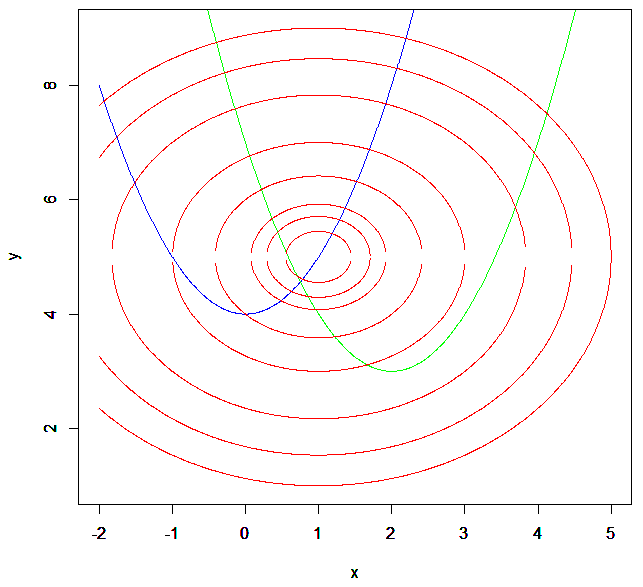
\includegraphics[scale=0.5]{q12}
\end{center}

A figura acima mostra que basta resolver o sistema de duas equações com ambas as restrições ativas. Ela foi gerada na linguagem R com o código abaixo.

\singlespacing
\footnotesize
\begin{verbatim}
 ex3 <- function(t) {
    return (4 + t^2)
 }

 ex4 <- function(t) {
    return (3 + (t - 2)^2)
 }
   
 # (x - 3)^2 + (y - 5)^2 = r
 ex5 <- function(x, r, sinal) {
    return (5 + sinal * sqrt(r - (x - 1)^2))
 }
   
 dev.off()
 Mx1 <- -2
 Mx2 <- 2
 My1 <- -3
 My2 <- 10
 N <- 1000
 x <- matrix(0, N)
 y <- matrix(0, N)
 z <- matrix(0, N)
 a <- matrix(0, 16, N)
 for (i in 1:N) {
    # t(1) = Mx1, t(N) = Mx2
    t <- (Mx2 - Mx1)/(N - 1) * (i - 1) + Mx1 
    x[i] <- t
    # t <- 1
    y[i] <- ex3(t)
    z[i] <- ex4(t)
    a[1, i] <- ex5(t, 0.2, 1)
    a[2, i] <- ex5(t, 0.2, -1)
    a[3, i] <- ex5(t, 0.5, 1)
    a[4, i] <- ex5(t, 0.5, -1)
    a[5, i] <- ex5(t, 0.8, 1)
    a[6, i] <- ex5(t, 0.8, -1)
    a[7, i] <- ex5(t, 2, 1)
    a[8, i] <- ex5(t, 2, -1)
    a[9, i] <- ex5(t, 4, 1)
    a[10, i] <- ex5(t, 4, -1)
    a[11, i] <- ex5(t, 8, 1)
    a[12, i] <- ex5(t, 8, -1)
    a[13, i] <- ex5(t, 12, 1)
    a[14, i] <- ex5(t, 12, -1)
    a[15, i] <- ex5(t, 16, 1)
    a[16, i] <- ex5(t, 16, -1)
 }
 plot(x,y,type = 'l',col='blue',xlim=c(Mx1,Mx2),ylim = c(My1,My2),xlab='x',ylab='y')
 par(new=T)
 plot(x,z,type = 'l',col='green',xlim=c(Mx1,Mx2),ylim = c(My1,My2),xlab='x',ylab='y')
 for (i in 1:16) {
   par(new=T)
   plot(x,a[i,],type = 'l',col='red',xlim=c(Mx1,Mx2),ylim = c(My1,My2),xlab='x',ylab='y')
 }
\end{verbatim}
\doublespacing
\normalsize

b) as condições de KKT. 

$g_1(x_1, x_2) = -x_1^2 + x_2 - 4 \le 0$; $\cfrac{\partial g_1}{\partial x_1} = -2x_1$; $\cfrac{\partial g_1}{\partial x_2} = 1$;

$g_2(x_1, x_2) = -(x_1 - 2)^2 + x_2 - 3 \le 0$; $\cfrac{\partial g_2}{\partial x_1} = -2(x_1 - 2)$; $\cfrac{\partial g_2}{\partial x_2} = 1$;

$\cfrac{\partial f}{\partial x_1} = 2(x_1 - 1)$; $\cfrac{\partial f}{\partial x_2} = 2(x_2 - 5)$;

\newpage
\singlespacing
Procuramos $\mu_1, \mu_2 > 0$ e a solução $x^* = x$ tais que:

\begin{align*}
  \nabla f + \mu_1 \nabla g_1 + \mu_2 \nabla g_2 &= 0\\
  2(x_1 - 1) - 2 \mu_1 x_1 + 2 \mu_2 (x_2 - 5) &= 0\\
  2(x_2 - 5) + \mu_1  + \mu_2 &= 0\\
  \mu_1 g_1 &= 0 \Rightarrow [\mu_1 = 0 \wedge g_1 < 0] \vee [\mu_1 \ne 0 \wedge g_1 = 0] \\
  \mu_2 g_2 &= 0 \Rightarrow [\mu_2 = 0 \wedge g_2 < 0] \vee [\mu_2 \ne 0 \wedge g_2 = 0] \\
  g_1 &\le 0\\
  g_2 &\le 0
\end{align*}

Caso $\mu_1 = \mu_2 = 0$, temos $x_1 = 1$ e $x_2 = 5$. Mas $g_2(1,5) = -1 + 5 - 3 > 0$. A solução não é factível.

\vspace{3mm}

Caso $\mu_1 = g_2 = 0$:

\begin{align*}
  2(x_1 - 1) + 2 \mu_2 (x_2 - 5) &= 0 \Rightarrow x_1 = 1 - \mu_2 (x_2 - 5) = 1 + 0.5 \mu_2^2 \\
  2(x_2 - 5) + \mu_2 &= 0 \Rightarrow x_2 = 5 - 0.5 \mu_2 \\
  x_2 &= 3 + (x_1 - 2)^2 \Rightarrow 2 - 0.5 \mu_2 = (0.5 \mu_2^2 - 1)^2 \Rightarrow \mu_2 = 2,\,x_1 = 3,\,x_2 = 4
\end{align*}

A solução é factível, mas não é o mínimo: $f(3,4) = 5$.

\vspace{3mm}

Caso $\mu_2 = g_1 = 0$:

\begin{align*}
  2(x_1 - 1) - 2 \mu_1 x_1 &= 0 \Rightarrow x_1 = \cfrac{1}{1 - \mu_1} \\
  2(x_2 - 5) + \mu_1 &= 0 \Rightarrow x_2 = 5 - 0.5 \mu_1 \\
  x_2 &= 4 + x_1^2 \Rightarrow 1 - 0.5 \mu_1 = \cfrac{1}{(1 - \mu_1)^2} \Rightarrow \mu_1 = 0,\,x_1 = 1,\,x_2 = 5\text{ novamente.}
\end{align*}

Caso $g_1 = g_2 = 0$:

\begin{align*}
  2(x_1 - 1) - 2 \mu_1 x_1 + 2 \mu_2 (x_2 - 5) &= 0\\
  2(x_2 - 5) + \mu_1  + \mu_2 &= 0\\
  x_2 &= 4 + x_1^2\\
  x_2 &= 3 + (x_1 - 2)^2 = 4 + x_1^2 \Rightarrow x_1 = \cfrac{3}{4} \Rightarrow x_2 = 4 + \cfrac{9}{16} = \cfrac{73}{16}
\end{align*}

$f\biggl(\cfrac{3}{4}, \cfrac{73}{16}\biggl) = \cfrac{65}{256}$. Mínimo.

\vspace{6mm}

Versão de 29/novembro/2021\footnote{Fora da caridade não há salvação.}  por Vinicius Claudino Ferraz.

\end{document}
